\section{Listas}


%%%%%%%%%%%%%%%%%%%%%%%%%%
\begin{frame}
\frametitle{Listas}
\begin{minipage}{0.47\textwidth}
    \begin{itemize}
        \item Definição de listas
        \item Representação
        \item Operadores
        \item Geração de listas
        \item Exemplos
    \end{itemize}
\end{minipage}
\begin{minipage}{0.5\textwidth}
\begin{figure}[ht!]
\begin{center}

\includegraphics[width=1.2\textwidth, height=0.40\textheight]{figures/logo_picat_alex.jpg}
\end{center}
\end{figure}
\end{minipage}
\end{frame}
%%%%%%%%%%%%%%%%%%%%%%%%%%



\begin{frame}[fragile]

    \frametitle{Listas}

   \begin{block}{}
     \begin{itemize}
      \item Requisito: conceito de recursividade, \textit{aterramento} etc,  dominados!
      
      \pause
      \item  Os conceitos são os próximos os das  LPs convencionais
           \pause 
     \item Essencialmente vamos computar sob uma árvore
         binária (\textcolor{green}{cada nó sempre tem duas ramificações})

           \pause 
      \item Lembrando que uma estrutura binária de árvore tem uma
      equivalência com uma árvore n-ária (ver livro de Estrutura de Dados)

           \pause 
       \item Logo,  listas são estruturas flexíveis e poderosas!

    \end{itemize}
    
    \end{block}
    
\end{frame}





\begin{frame}
 % \frametitle{Fluxo do Cálculo Recursivo}
\frametitle{Ilustrando uma Lista em Formato Binário}

\begin{figure}[!htb]
\centering
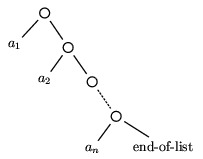
\includegraphics[width=.7\textwidth, height=0.650\textheight]{figures/ilustra-lista-01.jpg}
%\label{fig_ilustra_arv}
\caption{Uma estrutura  Lista -- Homogênea}
\end{figure}

\end{frame}


\begin{frame}
  \frametitle{Ilustrando  Listas e o Operador `\textbf{|}' (ou `\textbf{:}' da figura)}
\begin{figure}[!htb]
\centering
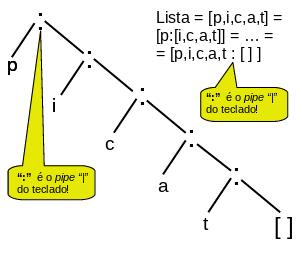
\includegraphics[width=.7\textwidth, height=0.650\textheight]{figures/lista-picat-01.jpg}
%\label{fig_arv_recurs_2}
\caption{Listas são inerentemente \textbf{recursivas}!}
\end{figure}
\end{frame}



\begin{frame}
 \frametitle{Exemplos de Listas}
\begin{figure}[!htb]
\centering
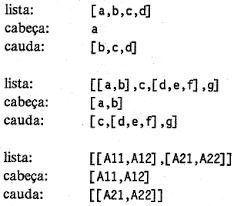
\includegraphics[width=.7\textwidth, height=0.650\textheight]{figures/exemplo_listas_01.jpg}
%\label{fig_arv_recurs_2}
%\caption{Fluxo Recursivo 2}
\end{figure}
\end{frame}



%%%%%%%%%%%%%%%%%%%%%%%%%%%%%%%%%%%%%%%%%%%%%%%%%%%%
\begin{frame}[fragile, allowframebreaks=0.9]
 \frametitle{Sintaxe das Listas}


\begin{block}{Definições iniciais (e recursivas)}
\begin{itemize}


\item Uma lista é uma sequência de termos (objetos)

\pause
\item Uma lista é uma estrutura de dados que representa
uma coleção de termos homogêneos

\item Como Picat a tipagem é dinâmica, o tipo só interessa quando
alguma ação é feita sobre ele, as listas em Picat podem
ser heterogêneas

\item Uma lista  apresenta uma hierarquia natural, internamente,
em \textcolor{magenta}{\textbf{cabeça}} de lista e sub-lista, até o fim da lista.

\end{itemize}
\end{block}
%\lbrack       left bracket [
%\rbrack       right bracket ]

\framebreak
\begin{block}{Notação:}
\begin{itemize}
   \item O símbolo ``\lbrack'' é usado para descrever o início de uma lista,
e ``\rbrack'' para o final da mesma;

   \item Exemplo: seja a lista \lbrack a, b, c, d \rbrack,  logo um predicado cujo
argumento seja algumas letras,  tem-se uma lista do tipo:\\
  \begin{itemize}
  \item letras(\lbrack  a, b, c, d \rbrack )
 \item Onde `a' é  o   \textit{cabeça} (primeiro elemento) da lista
 \item e \lbrack b, c, d \rbrack é uma \textit{sub-lista} que é uma lista!
  \end{itemize}

\item Os elementos de uma lista são lidos da esquerda para direita;

\item  A ``{\em sub-lista}'' \lbrack b,  c, d \rbrack é conhecida como  \textcolor{magenta}{resto} ou
\/ ``\textcolor{magenta}{{\em cauda}}'' da lista;
        
\item   Esta sub-lista é uma lista e toda definição segue-se recursivamente.
 \end{itemize} 

\end{block}


\framebreak
\begin{block}{Operador ``{\bf |}'':}

\begin{itemize}
  \item ``{\em  Como vamos distinguir de onde se encontra
a cabeça  da cauda da lista?}'' 

  \item Com as listas novos símbolos foram introduzidos, 
isto é, além dos delimitadores \lbrack \ldots \rbrack, há um 
 novo operador que \textbf{separa} 
 ou \textbf{define} quem é a elemento cabeça da lista e  cauda. 

  \item Este operador é conhecido como
 ``{\em pipe}'' (ou \textit{barra vertical}), simbolizado por ``{\bf |}'', que 
 separa  o lado esquerdo  da direita da lista. 
 
  \item  Esta separação  é necessário para se realizar os 
  \textit{casamentos de padrões} nas linguagens lógicas.

\end{itemize}
\end{block}

\framebreak
\begin{block}{Exemplos de \textcolor{magenta}{{\em \textbf{casamentos}}}:}

\begin{footnotesize}
\begin{verbatim}
 [ a, b, c, d ] = X
 [ X | b, c, d ]  =  [ a, b, c, d ]
 [ a | b, c, d ]  =  [ a, b, c, d ]
 [ a , b | c, d ]  =  [ a, b, c, d ]
 [ a , b , c | d ]  =  [ a, b, c, d ]
 [ a , b , c , d | [] ]  =  [ a, b, c, d ]
 [] = X
 [ [ a | b , c , d] ] = [ [ a , b , c , d ] ]
 [  a | b , c , [ d ] ] = [  a , b , c , [ d ] ]
 [  _ | b , c , [d ] ] = [  a , b , c , [ d ] ]
 [  a | Y ] = [  a , b , c ,  d ]
 [  a | _ ] = [  a , b , c ,  d ]
 [  a , b | c , d ] = [  X , Y | Z ]
 \end{verbatim}
\end{footnotesize}
\end{block}

\framebreak
\begin{block}{Contra-exemplos de \textcolor{magenta}{{\em \textbf{casamentos}}}:}

\begin{verbatim}
 [ a , b | [c, d] ]  !=  [ a, b, c, d ]
 [ [ a , b , c , d] ]  !=  [ a, b, c, d ]
 [  a , b , [ c ] , d, e ]  !=  [ a, b, c, d, e ]
 [ [ [ a ] | b , c , d] ] != [ [ a , b , c , d] ]
 \end{verbatim}

\end{block}

\framebreak
\begin{itemize}
  \item Estes  casamentos de termos de uma lista
  são também conhecidos  por \textcolor{magenta}{{\em matching}} 

\item  Devido ao fato de listas modelarem
qualquer estrutura de dados, invariavelmente, seu uso  é extensivo
há  problemas em geral (dos simples a complexos)

\item Porém, alguns cuidados no uso de predicados com \textcolor{magenta}{\textit{backtracking}}.
 Acompanhe os exemplos.

\item Os próximos exemplos encontram-se no arquivo: \textcolor{red}{\textbf{\url{../picat/listas.pi}}}

\end{itemize}


\end{frame}
%%%%%%%%%%%%%%%%%%%%%%

\begin{frame}[fragile]

\frametitle{Exemplos sobre Listas (e Implementações)}

\begin{enumerate}
  \item Comprimento de uma lista: retorna um valor numérico
  
  \pause
  \item Se um elemento $x$ pertence a lista: retorna um valor binário (\textit{true} ou \textit{false})


  \pause
  \item Adicionar um elemento $x$ em uma lista: retorna uma nova lista, o $x$ inserido nesta lista,
  se $x$ já estiver presente, não insira. Em resumo: insere $x$ em $L$ sem repetição.

  \pause
  \item Concatena duas listas: retorna uma terceira lista
  
\end{enumerate}

Em resumo: 4 métodos clássicos!

\end{frame}
%%%%%%%%%%%%%%%%%%%%%%

\begin{frame}[fragile, allowframebreaks=0.9]
\frametitle{Exemplo 01: encontrar o comprimento de uma lista}
 
\begin{itemize}
   \item O comprimento de uma lista é o comprimento de sua \textbf{sub-lista}, mais \textbf{um}
   \item O comprimento de uma lista vazia (\lbrack  \rbrack) é zero.
 \end{itemize} 
 
Em Picat, sob uma \underline{visão funcional}, este enunciado é escrito por:

\begin{verbatim}
comprimento_02( [ ] ) = 0.
comprimento_02([ _ | L ]) = N  => 
             N = 1 + comprimento_02( L ).
\end{verbatim}

\framebreak

Em Picat, sob uma \underline{visão lógica}, este predicado 
pode ser construído como:

\begin{verbatim}
comprimento_01([],N) ?=> N = 0. 
%%% em PROLOG, apenas comprimento_01([],0). PORQUÊ?
comprimento_01([_|L],N)  => 
             comprimento_01( L , Parcial ), 
             N = 1 + Parcial.
\end{verbatim}

\framebreak
Um {\em mapa de memória} é dado por:

\begin{center}
\begin{tabular}[c]{|c|c|c|c|c|c|}
\hline
& Regra & X & T & N & N = N+1\\\hline
compto([a,b,c,d],N) & \#2 & a & [b,c,d] & 3 $\rightarrow$ & 3+1$=$4\\\hline
compto([b,c,d],N) & \#2 & b & [c,d] & 2 $\rightarrow$ & $\nwarrow$ 2+1\\\hline
compto([c,d],N) & \#2 & c & [d] & 1 $\rightarrow$ & $\nwarrow$ 1+1\\\hline
compto([d],N) & \#2 & d & [] & 0 $\rightarrow$ & $\nwarrow$ 0+1\\\hline
compto([],N) & \#1 & -- & -- & -- & $\nwarrow$ 0\\\hline
\end{tabular}
\end{center}
 
 \end{frame}
%%%%%%%%%%%%%%%%%%%%%%%%%%%%%%%%%%%%%%%%%%%%%%%%%%%%%%%%%%%%%%%%%%%%

\begin{frame}[fragile, allowframebreaks=0.9]
\frametitle{Exemplo 02: verificar a pertinência de um objeto na lista}

\begin{itemize}
  \item Verifica se um dado objeto pertence há uma  lista
  \item Um método clássico -- muito usado
  \item Tem embutido no Picat: o \textit{menber}
\end{itemize}

Em Picat, sob uma \underline{visão funcional}, esta função é escrita por:

 \begin{verbatim}
pertence_02( _ , [ ]) = false. 
pertence_02( A, [A|_]) = true. 
% CUIDAR ... em funcoes nao hah ? em ?=> ... 
% sem backtracking em funcoes
pertence_02(A, [B|L]) = X => 
             A != B,
             X = pertence_02(A,L).
\end{verbatim}

%O interessante é observar a versatilidade 
%deste  predicado em várias situações:


\framebreak
Em Picat, sob uma \underline{visão lógica}, este predicado 
pode ser construído como:
\begin{verbatim}
pertence_01( A, [A|_]) ?=> true. 
% Again, backtracking CONTROLADO ... diferente do Prolog
pertence_01(A,[B|L])  => 
             A != B ,
             pertence_01(A,L).
\end{verbatim}

\end{frame}


\begin{frame}[fragile, allowframebreaks=0.9]
\frametitle{Exemplo 03: adicionar um elemento  em uma lista}

\begin{itemize}
  \item Um objeto é adicionado no início da lista (sem repeti\c{c}ão) caso este já
 esteja contido na lista, a lista original é a retornada:
%  \item 
\end{itemize}

Em Picat, sob uma \underline{visão funcional}, esta função é escrita por:
 
\begin{verbatim}
add_X_lista_02(X, [ ]) = [X]. 
add_X_lista_02(X, Y) = Z =>
          pertence_02(X, Y) = true,
          Z = Y ;
          Z = [ X | Y ].
\end{verbatim}


\framebreak
Em Picat, sob uma \underline{visão lógica}, este predicado 
pode ser construído como:
\begin{verbatim}

add_X_lista_01(X, [ ], Z )  ?=> Z = [X]. 
add_X_lista_01(X, Y, Z) ?=>
          pertence_01(X, Y),
          Z = Y .
add_X_lista_01(X, Y, Z) =>
          Z = [ X | Y ].

\end{verbatim}

\end{frame}




\begin{frame}[fragile, allowframebreaks=0.9]
\frametitle{Exemplo 04: união de duas listas}

\begin{itemize}
  \item O método de  união ou concatenação entre duas listas,
 resultando em uma terceira lista

 \item Este predicado é conhecido como \textit{append} ou \textit{concatena}. O \textit{append} está 
pronto na  biblioteca default do Picat

\item Há uma versão simplificada: \texttt{L3 = L1 \textbf{++} L2}

\end{itemize}

Em Picat, sob uma \underline{visão funcional}, esta função é escrita por:
\begin{verbatim}
uniao_02( [], X ) = X. 
uniao_02( [X|L1], L2 ) = L3 => 
                           L3 = [X | uniao_02( L1, L2 )].
\end{verbatim}

\framebreak

Em Picat, sob uma \underline{visão lógica}, este predicado 
pode ser construído como:

\begin{verbatim}
uniao_01( [] , X, Y ) ?=> Y = X. 
uniao_01( A , L2, R  ) =>  A = [X|L1] , 
                           R = [X|L3] , 
                           uniao_01( L1, L2, L3 ).
\end{verbatim}

\end{frame}


\begin{frame}[fragile]

\frametitle{Geração de  Listas -- \textit{list comprehension}}

\begin{block}{}
\begin{itemize}
  \item O conceito de \textit{list comprehension} veio da programação funcional
  \item Basicamente serve para criarmos ou gerarmos listas
  \pause
  \item Bastante útil e pode ser usada em qualquer parte de um código
  
\end{itemize}
\end{block}

\end{frame}


\begin{frame}[fragile]

\frametitle{Geração de  Listas -- \textit{list comprehension}}

Um \textit{list comprehension} tem o seguinte formato
na criação de listas:
\begin{tabbing}
aa \= aaa \= aaa \= aaa \= aaa \= aaa \= aaa \kill
\> \> \texttt{[$T$ : $E_1$ \texttt{in} $D_1$, $Cond_1$, $\ldots$, $E_n$ in $D_n$, $Cond_n$]} 
\end{tabbing}
\begin{itemize}
  \item $T$ é uma termo (uma expressão num caso genérico)
  \item $E_i$ é um padrão de iteração 
  \item $D_i$ é uma expressão de um valor composto, em geral um intervalo de domínio
  \item Opcionalmente,  condições $Cond_1$,$\ldots$,$Cond_n$  são chamados de \textit{termos}
  \item Esta geração de lista tem a seguinte interpretação: 
  \textit{toda tupla de valores $E_1 \in D_1$, $\ldots$, $E_n \in D_n$, 
  se as condições $Cond_i$ forem verdades, então o valor do termo $T$ 
  é adicionado na lista em construção}
\end{itemize}
\end{frame}


\begin{frame}[fragile]

\frametitle{Geração de  Listas -- \textit{list comprehension}}

Um vetor ou matrizes também pode 
ser construídos com um  \textit{array comprehension} e tem
o seguinte formato:
\begin{center}
\texttt{\{$T$ : $E_1$ \texttt{in} $D_1$, $Cond_1$, $\ldots$, $E_n$ in $D_n$, $Cond_n$\}} 
\end{center}

\pause
Isto é o mesmo como
%It is the same as:
\begin{center}
\texttt{to\_array([$T$ : $E_1$ \texttt{in} $D_1$, $Cond_1$, $\ldots$, $E_n$ in $D_n$, $Cond_n$])} 

\end{center}
\end{frame}


\begin{frame}[fragile]

\frametitle{Exemplos de \textit{list comprehension}}
\begin{footnotesize}
\begin{verbatim}
main => Status = command("clear") ,
		printf("====================================== %d", Status),
    L0 = [I :  I in 10..20],
    L1 = [I :  I in 10..2..20],
    L2 = [I :  I in 1..20, I>10, I<20],
    L3 = [(A,I) : A in [a,b], I in 1..10, I mod 2 == 0],
    L4 = [(I,J,K) :  I in 1..2, J in 3..7, K in 1..10, I+J < K],
    printf("\n L0 : %w " , L0),
    printf("\n L1 : %w " , L1),
    printf("\n L2 : %w " , L2),
    printf("\n L3 : %w " , L3),
    printf("\n L4 : %w " , L4),
    printf("\n FIM\n").
    
%  $ picat geracao_listas.pi    
\end{verbatim}
\end{footnotesize}
\end{frame}



\begin{frame}[fragile]

\frametitle{Saída: \textit{list comprehension}}

\begin{footnotesize}
\begin{verbatim}
====================================== 0
 L0 : [10,11,12,13,14,15,16,17,18,19,20] 
 L1 : [10,12,14,16,18,20] 
 L2 : [11,12,13,14,15,16,17,18,19] 
 L3 : [(a,2),(a,4),(a,6),(a,8),(a,10),(b,2),(b,4),(b,6),(b,8),(b,10)] 
 L4 : [(1,3,5),(1,3,6),(1,3,7),(1,3,8),(1,3,9),(1,3,10),(1,4,6),
 (1,4,7),(1,4,8),(1,4,9),(1,4,10),(1,5,7),(1,5,8),(1,5,9),(1,5,10),(1,6,8),
 (1,6,9),(1,6,10),(1,7,9),(1,7,10),(2,3,6),(2,3,7),(2,3,8),(2,3,9),(2,3,10),
 (2,4,7),(2,4,8),(2,4,9),(2,4,10),(2,5,8),(2,5,9),(2,5,10),
 (2,6,9),(2,6,10),(2,7,10)] 
 FIM
\end{verbatim}
\end{footnotesize}

\textcolor{red}{L4 ... \textit{cortada}}
\end{frame}



%%%%%%%%%%%%%

\begin{frame}[fragile]
\frametitle{Concluindo Listas}

\begin{block}{}
\begin{itemize}
  \item Há muitos predicados e funções prontas sobre listas nos módulos do Picat
  \pause
  \item Contudo, se aprende sobre listas, fazendo \textcolor{magenta}{\textbf{muitos}} métodos
    \pause
  \item A recursividade em sua modelagem, define a \textcolor{magenta}{metodologia de se \textit{programar em lógica}}
    \pause
  \item Exercitar-se para aprender os detalhes!
    \pause
  \item Usar as listas como estrutura base em problemas complexos
  
     \pause
  \item Próxima na aula: buscas (\textcolor{magenta}{\textbf{uso extensivo de listas}})
  
\end{itemize}

\end{block}

\end{frame}
